\documentclass[a4paper,11pt]{article}

\usepackage{listings}
\usepackage{enumerate}
\usepackage{graphicx} % Required for including images
\usepackage[font=small,labelfont=bf]{caption}
\usepackage{geometry}

\title{The benefits of an extended feature space in a machine learning bot for the game Schnapsen}
\date{January 25, 2018}
\author{Lucas Faijdherbe, Daan Schrage and Ruben van der Ham\\\\
	\small Intelligent Systems\\
	\small Vrije Universiteit Amsterdam}

\begin{document}
\maketitle
\clearpage

\begin{abstract}
This paper examines the effect of extended and narrowed feature spaces on logistic regression machine learning bot. To illustrate this, 5 different machine learning bots were created: two bots with narrowed feature spaces, three bots with extended feature spaces. These bots were trained multiple times, and played multiple tournaments against multiple other bots. The results are.. 
\end{abstract}

\section{Introduction}
Artificial Intelligence is becoming a huge subject, and we see it appearing more and more in daily life: voice assistants on smartphones, self-driving Tesla's, AlphaGo defeating Go masters, and so on. within the field, we can make a distinction between strong and weak AI [1]: \textit{weak AI} is focused on mastering problems in one limited area, whereas \textit{strong AI} is considered to be Artificial Intelligence with \textit{actual} intelligence, and even self-awareness. For this paper, we will concentrate on weak AI in the game of Schnapsen. The weak-AI in this game are machine-learning bots. In this paper, we will specifically focus on the feature spaces of these machine-learning bots, and how the differences in features affect performance of the bots. In section 2 we will describe Schnapsen and the Schnapsen framework in detail, alongside the non-AI bots that have already been implemented. The research question will be described in section 3. In section 4, we will talk about the machine-learning (AI) bots, and the research setup. Consequently in section 5 we will describe the results of the experiment, and in section 6 we will elaborate on our findings. Finally, in section 7 we will draw our conclusion.

\section{Background Information}
\subsection{Schnapsen}
Schnapsen is an Austrian card game, played with 20 cards; Only the Jacks, Queens, Kings, 10s and Aces are in the deck. The goal of the game is to win tricks, and to be the first player to score 66 points. Each game has a trump suit, which is determined randomly. A card from the trump suit lets you automatically win the trick, provided that there is no higher trump card in the game.

The game has a multi-agent (we have an opponent), deterministic (the environment is determined by the current state and executed action), static (the environment does not change when an agent is choosing an action) and discrete (the game is turn-based) environment. The game consists of two phases: In phase one, when there are still cards in stock, we have an imperfect information game. In phase two, when the stock is depleted, we have a perfect information game, since we know exactly what the cards of our opponent are. The point count in the game is as follows: \\ \\
\noindent
\begin{tabular}{l l l l l}
\textbf{J} & \textbf{Q} & \textbf{K} & \textbf{10} & \textbf{A} \\
2 & 3 & 4 & 10 & 11 \\
\end{tabular} \\

\noindent
A lot of points can also be won by marriages. If the player is leading the trick and has a king or a queen of the same suit, it can play one card, and show the other, so the opponent knows that there is a marriage.\\ \\
\noindent
\begin{tabular} {c c}
\textbf{Normal marriage (non-trump suit)} & \textbf{Royal marriage (trump suit)} \\
20 & 40 \\
\end{tabular}\\

\noindent
The game starts in phase one, an imperfect-information game. Each agent has 5 cards. Player 1 plays a card, thereby determining the suit that has to be played. To win the trick, player 2 has to play a higher-ranking card from the same suit, or a trump card. Player 2 does not have to follow suit in phase 1, but he/she will lose the trick in that case. The winner of the trick now becomes player one and gets the cards, with the amount of points the two cards represent. This goes on until the stock is depleted; then we enter phase 2, a perfect-information game. Player 2 now has to follow suit. If it cannot do that, the player has to trump, and otherwise play any card. If a player reaches 66 points or more, the game is over.

\subsection{Intelligent Systems Schnapsen Framework}
An API in Python has been provided, together with a framework for the Schnapsen game. Furthermore, we  have two scripts: one where bots can play against each other in a single game where all moves in the game can be seen, and a script where bots play a tournament against each other - with a specifiable number of games to be played - and where the number of won games per robot can be seen. There are already multiple bots present in the framework to play against:
\begin{description}
\item [Minimax / Alphabeta:] This bot only works in a perfect-information game (phase 2 of Schnapsen). It recursively looks through all the states, and decides what the best move to play will be, provided that the opponent plays optimally, and will try to minimize the outcome of the game for the player.
\item [Bully:] Plays by a defined set of rules. If it has a trump card, it will play that. Otherwise, it will play a card of the same suit player 1 played. If it cannot do either of those things, it will play the highest ranking card of any suit.
\item [Rand:] Chooses a random move out of all of the legal moves, and plays that.
\item [Rdeep:] Functions quite like a Monte-Carlo sampling bot. It looks through multiple states, and averages the heuristics of a state, thereby ranking the moves. It then picks one of the highest ranking moves to play.
\item [KBbot:] Logical reasoning bot. The strategy can be defined in propositional logic. The current strategy of the bot is to always play cheap cards (i.e kings, queens, jacks) first.
\end{description}

\subsection{Machine Learning Bots}
For this paper, we will use machine learning bots. These bots use a logistic regression algorithm to create the model. The model estimates to probability of a certain response based on on or more features. [2] The model can be retrieved by training the bot against another player. The bot will use the model when playing the actual games. For more information on our implementation of the machine learning bots, refer to section 4.


\clearpage
\section{Research Question}
In our research, we want to find \textit{what feature set will improve the machine learning bot's performance the most in the game of Schnapsen}. With improve the most, we mean as seen from the baseline. There is already a machine learning bot present, which will act as this base line. This bot has, what we will call the \textit{default feature space}- provided by the framework.  \\

\noindent
The \textit{default feature space} contains the following features:
\begin{itemize}
\item Perspective information
\item Player 1's point count
\item Player 2's point count
\item Player 1's pending points
\item Player 2's pending points
\item The trump suit
\item The phase
\item The stock size
\item The leader
\item Whose turn it is currently
\item The played card of the opponent
\end{itemize}



\noindent
Our goal is to build multiple bots machine learning bots, both with extended feature spaces and narrower feature spaces, and see which bot will improve most in relation to the default machine-learning bot. Our hypothesis is that the bots with an extended feature space will have a better performance the bots with a narrower feature space, and that the extended feature space bots will perform better than the default bot, where the narrow feature space will perform worse. This is because the narrowing of the feature space can cause underfitting, where the model 'cannot capture the underlying structure of the data'[3] increasing the chance of making a wrong prediction. Consequently, extending the feature space can cause overfitting, where the model has more features than the data needs, which can also lead to making the wrong predictions.


\clearpage
\section{Experimental setup}
For the purpose of our research, we created 5 machine-learning bots accompanying the original machine-learning bot, each competing in multiple 120 game Schnapsen tournaments against each individual non-learning bot. All bots were trained and tested in the same way. Below, we will give an overview of the bots and the changes made with respect to the default machine-learning bot. For the whole overview, refer to appendix A. After that, we will describe the testing procedure.

\subsection{The bots}
The non- learning opponents were Rand, Bully and Rdeep. The learning bots we created were:
\begin{description}
\item [ml\_minimal:] This bot has the smallest feature space of all: only the perspective and the point count of both player 1 and player 2 as features. We wanted to see if a bot can still perform well, even if it just has minimal amount of information about the game state.

\item [ml\_stripped:] ml\_stripped has almost all the features of the \textit{default feature space} except for both players pending points and trumpsuit id.

\item [ml:] This ml bot is provided by the framework and consists of the  \textit{default feature space} 

\item [ml\_enriched:]  This bot has a slightly extended feature space in comparison to the original ml-bot. The following features were added to the feature space:
\begin{itemize}
\item Both player's points squared
\item Both player's pending points squared
\item Both player's points cubed
\item Both player's pending points cubed
\end{itemize}
These features were added to go more to a design-matrix like feature space. Since the amount of points a player has are important for the game, we chose to focus solely on this.

\item [ml\_advanced:] 
This bot has a more extended feature space in addition to the \textit{default feature space}. Added are: 
\begin{itemize}
\item Difference between points
\item Difference between pending points
\item Trump card ratio in hand
\item High card ratio in hand (10/A's)
\item Number of trump cards in hand in phase 2
\item Number of cards with same suit as opponents played suit
\item Number of points in hand (squared)
\end{itemize}
This is the bot where we chose to add more of our own thought of features. Point difference was added, since this is a good indicator if a player is leading the game by a high margin. Furthermore, we chose to focus on both trump and high-ranking cards in the hand. The more you have, the better it is. The number of trump cards in phase 2 is also important: If you still got all your trump cards in phase 2 of the game, you have a high chance of beating your opponent. Furthermore the number of cards with same suit as opponents played suit feature was added, alongside the number of points in the player hand squared feature.

\item[ml\_combined:] This bot has the most extended feature space. It combines the features of ml\_enriched and ml\_advanced.
\end{description}
\subsection{The testing procedure}

Each learning bot played a total of 9 tournaments with 3 different models against each non-learning bot.
The testing procedure was as follows:
\begin{itemize}
\item Training
\item 120 Game tournament
\item 120 Game tournament
\item 120 Game tournament
\end{itemize}

This procedure was repeated twice to reach the total of 9 tournaments respectively. The testing only occurred between learning and non-learning bots.  The learning bots did not compete against each other.  In case of Rand and Bully, each training process consisted of 100,000 observations of the (non-learning) opponent. Rdeep was only observed 10,000 times during training, since training this bot takes a substantial amount of time. The margin of error we adhere is 5\%.
\clearpage
\section{Results}
The tournament results are presented in Table 1. 

\setlength{\leftmargin}{0pt}
\begin{center}
  \begin{tabular}{ | l | l l | l l | l l | |l l | }
     \hline
      & \textbf{rand} & & \textbf{bully} & & \textbf{rdeep} & & \textbf{Total} & \\
      & wins & losses & wins & losses & wins & losses  & wins & losses \\ \hline
      ml\_minimal & 843 & 237 & 837 & 243 & 348 & 732 & 2028 & 1212 \\ \hline
      ml\_stripped & 736 & 344 & 843 & 237 & 283 & 797 & 1862 & 1378 \\ \hline
      ml & 866 & 214 & 876 & 204 & 257 & 823 & 1999 & 1241 \\ \hline 
      ml\_enriched & 881 & 119 & 772 & 308 & 284 & 798 & 1937 & 1303 \\ \hline
      ml\_advanced  & 856 & 224 & 808 & 272 & 292 & 788 & 1956 & 1284 \\ \hline
      ml\_combined & 949 & 131 & 759 & 321 & 274 & 806  & 1982 & 1258\\ \hline
  \end{tabular}
\end{center}
\textbf{Table 1}: Overview of tournament wins and losses per ml-bot. \\

\begin{center}
\begin{tabular}{| r | r | r | r || r |}
\hline
      & \textbf{rand} & \textbf{bully} & \textbf{rdeep} & \textbf{Total} \\ \hline
      ml\_minimal & -2,65\% & -4,45\% & +35,4\% & \textbf{+1,45\%}   \\ \hline
      ml\_stripped & -15\% & -3,76\% & +10,11\% & \textbf{-6,85\%}  \\ \hline
      ml\_enriched & +1,73\% & -11,87\% & +10,5\% & \textbf{-3,10\%} \\ \hline
      ml\_advanced & -1,15\% & -7,76\% & +13,6\%& \textbf{-2,15\%}  \\ \hline
      ml\_combined & +9,58\% & -13,35\% & +6,61\% & \textbf{-0,85\%}  \\ \hline \hline
      Average improvement & \textbf{-1,5\%} & \textbf{-8,24\%} & \textbf{+15,24\%} &\textbf{-2,3\%} \\ \hline
\end{tabular} \\
\end{center}

\textbf{Table 2}: Improvement over ml. \\
\begin{center}
\begin{tabular}{| r | r | r | r |}
\hline
      & \textbf{rand} & \textbf{bully} & \textbf{rdeep}\\ \hline
      Standard deviation & 0.0652 & 0.0432 & 0.0280    \\ \hline
\end{tabular} \\
\end{center}

\textbf{Table 3}: \textit{Standard deviation} of the mean of the 9 tournaments for each bot. \\

\begin{center}
\begin{minipage}{0.49\linewidth}
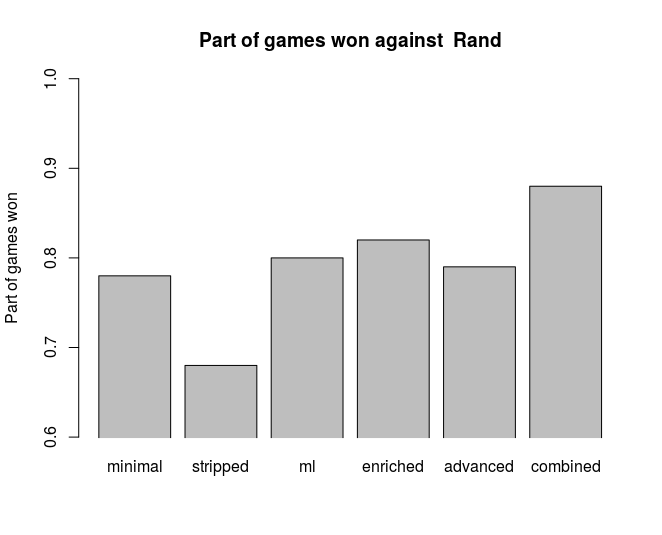
\includegraphics[width=\linewidth]{images/barplotRand.png}
\captionof{figure}{Part of games won against Rand}
\end{minipage}
\hfill
\begin{minipage}{0.49\linewidth}
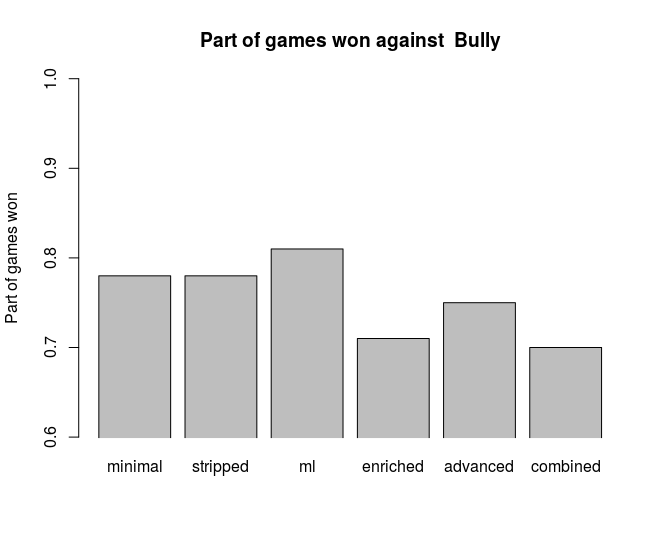
\includegraphics[width=\linewidth]{images/barplotBully.png}
\captionof{figure}{Part of games won against Bully}
\end{minipage}
      \\ %extra line for space
\begin{minipage}{0.49\linewidth}
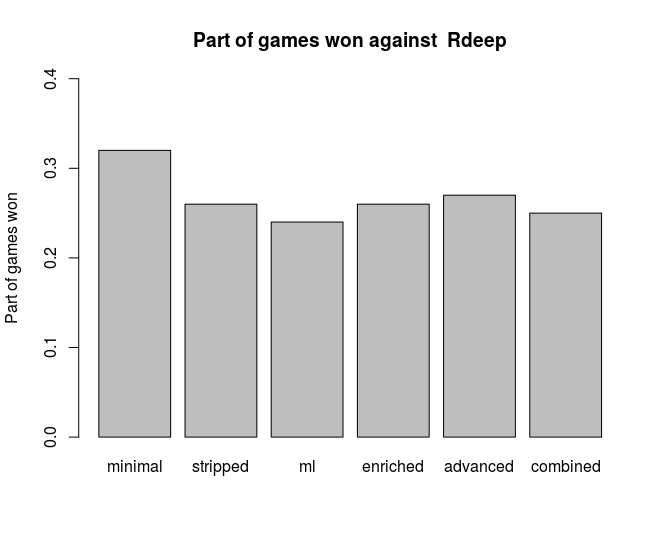
\includegraphics[width=\linewidth]{images/barplotRdeep.png}
\captionof{figure}{Part of games won against Rdeep (please notice the Y-axis)}
\end{minipage}
\end{center}

\section{Findings}

\subsection*{Against Rand}
There are a few notable things when comparing the performance of our bots. Firstly, while both ml\_minimal and ml\_stripped performed slightly worse that the stock ml bot, as was expected, ml\_stripped actually performs worse than ml\_minimal. Despite the latter of the two having the smallest feature set. However, the differences are below 5\% and therefore within the margin of error. Secondly, stripping away most of the feature set in ml\_minimal only led to a relatively small performance loss. Lastly, ml\_enriched and ml\_advanced perform, respectively, a little better and a little worse when compared to the stock ml bot. However, when we combined the feature sets of these two bots in ml\_combined, it led to an performance increase of almost 10\% compared to the stock ml bot. In short, the bots with the larger feature spaces did perform relatively better against rand.

\subsection*{Against Bully}

Notable for the results of the tournaments against the bully bot are the following points. First of all, the stock ml bot performed the best of all bots. In figure 2 this is clearly noticable. Secondly,  ml\_stripped and ml\_minimal peformed comparable to ml bot. Therefore, we may conclude the smaller feature spaces do not cause a heavy impact on the performance of a learning bot. The last and most remarkable finding is the peformance of the ml\_enriched and ml\_combined bots. All bots with larger feature spaces peformed worse than ml bot. However, ml\_enriched and ml\_combined performed the worst with a performance decrease of approximately 9\%.


\subsection*{Against Rdeep}
The \textit{standard deviation} of the mean of the 9 tournaments for each bot against rdeep is 0.0280. This number is the lowest of all the non-learning bots and is clearly confirmed by the barplot in figure 3. Rdeep won the majority of the games, which results in a low diversity of winning scores among the learning bots. The worst performer was, surprisingly, the stock ml bot. Although the variance in the winning scores is low, the ml\_minimal bot performs clearly better against rdeep. Compared to the other learning bots, ml\_minimal performs approximately 25\% better. Also remarkable is the relatively low score of ml\_combined with the most features of all. The other bots containing a larger feature space did perform slightly better than the stock ml bot, although this is all within the margin of error.  Summarized, the bots with the smallest featurespaces seemed to perform the best against rdeep.







\section{Conclusion}
Performance is different per bot, and we can not say a lot since we do not have the data to do so , not enough data blabalablalbalalb





\section{References}
1. http://humanparagon.com/strong-and-weak-ai/
2. https://towardsdatascience.com/machine-learning-part-3-logistics-regression-9d890928680f
3. https://en.wikipedia.org/wiki/Overfitting

\clearpage
\section{Appendix}
\subsection{Overview of machine-learning bots' feature spaces}
\begin{description}
\item[ml\_minimal]
\begin{itemize}
\item Perspective information
\item Player 1's point count
\item Player 2's point count
\end{itemize}
\subsection{ml\_stripped}
\begin{itemize}
\item Perspective information
\item Player 1's point count
\item Player 2's point count
\item The phase
\item The stock size
\item The leader
\item Whose turn it is currently
\item The played card of the opponent
\end{itemize}
\subsection{ml\_enriched}
\begin{itemize}
\item Perspective information
\item Player 1's point count
\item Player 1's point count squared
\item Player 1's point count cubed
\item Player 2's point count
\item Player 2's point count squared
\item Player 2's point count cubed
\item Player 1's pending points
\item Player 1's pending points squared
\item Player 1's pending points cubed
\item Player 2's pending points
\item Player 2's pending points squared
\item Player 2's pending points cubed
\item The trump suit
\item The phase
\item The stock size
\item The leader
\item Whose turn it is currently
\item The played card of the opponent
\end{itemize}
\subsection{ml\_advanced}
\begin{itemize}
\item Perspective information
\item Player 1's point count
\item Player 2's point count
\item Player 1's pending points
\item Player 2's pending points
\item Difference between player 1 and player 2's point count
\item Difference between player 1 and player 2's pending point count
\item The trump suit
\item Trump card ratio (Number of trump cards in hand / total number of cards in hand * 100)
\item High-ranking card ratio (Number of 10's and A's in hand / total number of cards in hand * 100)
\item The phase
\item Number of trump cards in hand in phase 2
\item The stock size
\item The leader
\item Whose turn it is currently
\item The played card of the opponent
\item Number of cards in same suit as opponent's played suit in hand.
\item Number of points in hand squared ($card1^2$ + $card2^2$ ...)
\end{itemize}

\subsection{ml\_combined}
\begin{itemize}
\item Perspective information
\item Player 1's point count
\item Player 1's point count squared
\item Player 1's point count cubed
\item Player 2's point count
\item Player 2's point count squared
\item Player 2's point count cubed
\item Player 1's pending points
\item Player 1's pending points squared
\item Player 1's pending points cubed
\item Player 2's pending points
\item Player 2's pending points squared
\item Player 2's pending points cubed
\item Difference between player 1 and player 2's point count
\item Difference between player 1 and player 2's pending point count
\item The trump suit
\item Trump card ratio (Number of trump cards in hand / total number of cards in hand * 100)
\item High-ranking card ratio (Number of 10's and A's in hand / total number of cards in hand * 100)
\item The phase
\item Number of trump cards in hand in phase 2
\item The stock size
\item The leader
\item Whose turn it is currently
\item The played card of the opponent
\item Number of cards in same suit as opponent's played suit in hand.
\item Number of points in hand squared ($card1^2$ + $card2^2$ ...)
\end{itemize}
\end{description}
\section{Worksheet I}
\begin{enumerate}

\item The \textit{rdeep} bot performs best, winning 20 out of 30 games. \\
Output:
\begin{lstlisting}[language=bash]
Results:
bot <bots.rand.rand.Bot instance at 0x101a70fc8>: 7 wins
bot <bots.bully.bully.Bot instance at 0x101a71098>: 3 wins
bot <bots.rdeep.rdeep.Bot instance at 0x101a71170>: 20 wins
\end{lstlisting}

\item The bully bot operates as follows:
\begin{itemize}
\item If it has a trump card, it will play that.
\item If it does not have a trump card, it will play a card from the same suit
\item If it cannot do either of those things, it will choose the highest ranking card of any suit.
\end{itemize}

\item Using this strategy means that you will try to get as many points as possible each move. However, this might also mean that early in the game, the bot will play valuable cards in order to get a high point ratio, but later in the game it has no good cards left. 

\item Have the bots complete a large number of tournaments (preferably n > 30), see if the rdeep bot still outperforms the rand bot, and how big the difference in wins is. If there is a significant difference, we can assume that rdeep is better than rand.

\item MyBot implementation:
It plays any available trump card first. If none is available it picks a random card.

\begin{lstlisting}[language=bash]
def get_move(self, state):
        moves = state.moves()
        return get_trump_card(moves,state)
def get_trump_card(moves,state):
    randomChoice = random.choice(moves)
    counter = 0
    if randomChoice == None:
        print "NONE FOUND"
    if moves == None:
        print "None available"
        return None
    while True:
        randomChoice = random.choice(moves)
        counter +=1
        if randomChoice == None:
            print "NONE returned"
            return randomChoice
        try:
            if util.get_suit(randomChoice[0]) 
            == State.get_trump_suit(state):
                #print "Playing trump card"
                return randomChoice
        except:
            #print "KEY ERROR"
            pass
        if counter > 40 and not randomChoice == None:
            #print "Playing normal card"
            return randomChoice
    return randomChoice
\end{lstlisting}

When no legal moves are to be made except the best trump card you have no legal moves when you  remove the trump card from the list of legal moves. In that case the python program expects a move but it gets a return type "None". That's why it raises an error.

Output:
\begin{lstlisting}[language=bash]
Results:
    bot <bots.rand.rand.Bot instance at 0x7fe73586fab8>: 25 wins
    bot <bots.mybot.mybot.Bot instance at 0x7fe73587a440>: 45 wins
\end{lstlisting}

\item The heat map:
- Insert pdf here - This heatmap means:
If player 2 has a high non-move probability, this is better for player 1 if player 1 has a low-non move probability. Both players seem to have a good value if the non-move probability is around 0.4 - 0.6.

\item The added line:
\begin{lstlisting}[language=bash]
value, move = self.value(next_state, depth + 1)
\end{lstlisting}
Output:
\begin{lstlisting}[language=bash]
python tournament.py -p rand,minimax -s 2 -r 10
Playing 10 games:
Played 1 out of 10 games (10%): [0, 1] 
Played 2 out of 10 games (20%): [0, 2] 
Played 3 out of 10 games (30%): [0, 3] 
Played 4 out of 10 games (40%): [0, 4] 
Played 5 out of 10 games (50%): [1, 4] 
Played 6 out of 10 games (60%): [2, 4] 
Played 7 out of 10 games (70%): [2, 5] 
Played 8 out of 10 games (80%): [3, 5] 
Played 9 out of 10 games (90%): [4, 5] 
Played 10 out of 10 games (100%): [4, 6] 
Results:
bot <bots.rand.rand.Bot instance at 0x102a70f80>: 4 wins
bot <bots.minimax.minimax.Bot instance at 0x102a731b8>: 6 wins
\end{lstlisting}

\item The added code:


It creates one instance for each bot, minimax and alphabeta. Then in generates a state, and it does a few random moves. It measures the time to get the next move from both the minimax and alphabeta, then it compares the outcomes. If they are equal it will print "Agreed." else it will display the answers of both bots. This process is repeated a few times.
Even though the code is right, the checking program does not behave correctly. That's why we do not have a valid output.

\item The heuristic is a value between -1.0 and 1.0, derived from the point ratio of the current player. If the player has a 1.0 value, the player has a definite win. If the value is -1.0, the opponent has a definite win.

We came up with, the ratio of trump cards in hand, it turned out to be a horrible heuristic. Holding on to your trumps seems to be a bad tactic. Therefore we tried ditching trumps as soon as possible, this lead to somewhat better results, but random was still a better bot in the end. 

\end{enumerate}
\section{Worksheet II}
\begin{enumerate}
\item The added clause that makes the knowledge base unsatisfiable:
\begin{lstlisting}[language=bash]
kb.add_clause(~B, ~C)
\end{lstlisting}

\item The three clauses converted to CNF:
\begin{itemize}
\item A V B
\item -B V A
\item -A V C
\item -A V D
\end{itemize}
The code that creates the variables and the knowledge base:
\begin{lstlisting}[language=bash]
# Define our symbols
A = Boolean('A')
B = Boolean('B')
C = Boolean('C')
D = Boolean('D')

# Create a new knowledge base
kb = KB()

# Add clauses
kb.add_clause(A, B)
kb.add_clause(~B, A)
kb.add_clause(~A, C)
kb.add_clause(~A, D)
\end{lstlisting}
Because the knowledge base entails A \& C \& D, all three have to be true. For now, the model has two solutions:
\begin{lstlisting}[language=bash]
{A: True, C: True, B: False, D: True}
{A: True, C: True, B: True, D: True}
\end{lstlisting}
B can be whatever it wants, but A, B and D have to be true.

\item Three constraints have to be met:
\begin{enumerate}[I]
\item $X = Y$
\item $X + Y > 2$
\item $X + Y < 5$
\end{enumerate}
The model is satisfiable, as long as: 
$1 < x < 2.5$ and $1 < y < 2.5$

\item We now have three models:
\begin{lstlisting}[language=bash]
(a) [x = y] = True, [x + y > 2] = True, [x + y < 5] = True
(b) [x = y] = True, [x + y > 2] = True, [x + y < 5] = False
(c) [x = y] = True, [x + y > 2] = False, [x + y < 5] = True
\end{lstlisting}

The three constraints per model: \\\\
(a) This model already has three constraints. \\
(b) Only the last clause has to change, namely to $[x + y >=5] $= True\\
(c) Only the second clause has to change, namely to$ [x + y <= 2]$ = True.\\

Now we end up with this:
\begin{lstlisting}[language=bash]
(a) [x = y] = True, [x + y > 2] = True, [x + y < 5] = True
(b) [x = y] = True, [x + y > 2] = True, [x + y >= 5] = True
(c) [x = y] = True, [x + y <= 2] = True, [x + y < 5] = True
\end{lstlisting}

\item What we want, is to find points on the line $x = y$, where the points either lie between $x + y > -5$ and $x + y < -2$, or where the points lie between $x + y > 2$ and $x + y < 5$.

The clauses we need to add are:
\begin{itemize}
\item $x == y$
\item $x + y > 2 V  x + y < -2$
\item $x + y > -5 V  x + y < 5$
\item $x + y > - 5 V  x + y > 2$
\item $x + y < -2 V  x + y < 5$
\end{itemize}

The code:
\begin{lstlisting}[language=bash]
# Define our integer symbols
x = Integer('x')
y = Integer('y')

q = x == y
a = x + y > 2
b = x + y < 5
c = x + y < -2
d = x + y > -5

kb = KB()

kb.add_clause(q)
kb.add_clause(a, c)
kb.add_clause(a, d)
kb.add_clause(b, c)
kb.add_clause(b, d)
\end{lstlisting}

\item 6)The playing ace strategy work:

\begin{lstlisting}[language=bash]
kb.add_clause(A0)
kb.add_clause(A5)
kb.add_clause(A10)
kb.add_clause(A15)


#PLAY ACE STRATEGY
kb.add_clause(~A0, PA0)
kb.add_clause(~A5, PA5)
kb.add_clause(~A10, PA10)
kb.add_clause(~A15, PA15)
kb.add_clause(~PA0, A0)
kb.add_clause(~PA5, A5)
kb.add_clause(~PA10, A10)
kb.add_clause(~PA15, A15)
\end{lstlisting}

When adding: 
\begin{lstlisting}[language=bash]
kb.add_clause(~PA0)
\end{lstlisting}
The statisfiability with the KB fails, therefore we know PA0 is entailed by the KB

\item We implemented the PlayCheap strategy:

\item Game output

\item 
\end{enumerate}
\section{Worksheet III}
\begin{enumerate}
\item The added code:
\begin{lstlisting}[language=bash]
value = self.heuristic(next_state)

p1_points = state.get_points(1)

p2_points = state.get_points(2)

p1_pending_points = state.get_pending_points(1)

p2_pending_points = state.get_pending_points(2)

trump_suit = state.get_trump_suit()

phase = state.get_phase()

stock_size = state.get_stock_size()

leader = state.leader()

whose_turn = state.whose_turn()

opponents_played_card = state.get_opponents_played_card()
\end{lstlisting}
The result of the played tournament against rand and bully:
\begin{lstlisting}[language=bash]
bot <bots.ml.ml.Bot instance at 0x102271290>: 16 wins
bot <bots.rand.rand.Bot instance at 0x1022711b8>: 4 wins
bot <bots.bully.bully.Bot instance at 0x1059b71b8>: 10 wins
\end{lstlisting}

\item We let the mlbot learn by playing against rdeep. But since the games took way longer than the games of mlbot vs rand, we set the number of games to 1000 (Which still took quite some time).

We get a lower output now:
\begin{lstlisting}[language=bash]
bot <bots.ml.ml.Bot instance at 0x102a73248>: 15 wins
bot <bots.rand.rand.Bot instance at 0x102a73170>: 7 wins
bot <bots.bully.bully.Bot instance at 0x10599df80>: 8 wins
\end{lstlisting}

ML now wins 15 times, where it won 16 times on the first tournament. This might have to do with the training set being smaller, and it was trained against rdeep, which does not compete in the tournament. However, the difference is not comparably worse.

We decided to train the mlbot again against rdeep, but now with 5000 games. 
Even after this long wait, the robot does not play significantly better or worse.

\begin{lstlisting}[language=bash]
bot <bots.ml.ml.Bot instance at 0x102a71248>: 14 wins
bot <bots.rand.rand.Bot instance at 0x102a71170>: 5 wins
bot <bots.rdeep.rdeep.Bot instance at 0x105aa2cf8>: 11 wins
\end{lstlisting}

\item We created three ml bots:
\begin{itemize}
\item The first one was trained on rdeep
\item The second one was trained on rand
\item The third one was trained on the second bot.
\end{itemize}

We played a tournament with 300 games in total. The results:
\begin{lstlisting}[language=bash]
    bot <bots.ml.ml.Bot instance at 0x10ad81ef0>: 92 wins
    bot <bots.ml.ml.Bot instance at 0x10ad81f80>: 99 wins
    bot <bots.ml.ml.Bot instance at 0x10b80cb00>: 109 wins
\end{lstlisting}
As you can see, bot 3 only performed a bit better than the other two, but there is no really significant difference between the bots.

\item For added features, read this research paper. It's all about added features.

\end{enumerate}
\end{document}
